 \chapter{Introduction}
\label{intro}


\section{Embedded Systems and Energy Consumption}

Embedded systems are usually designed to perform a specific tasks and often consist of domain-specific hardware.
For example, typical embedded systems use optimized processing cores to perform signal processing instead of using general purpose CPUs.
Some examples of embedded systems include TV sets, cellular phones, MP3 players, smart cameras, wireless access points and printers. 
An embedded system is designed with strong requirements regarding size, performance and power consumption.
The market demand is towards smaller and lighter devices.
The ever-progressing semiconductor processing technique has dramatically increased the number of transistors on a single chip, which makes today's hardware increasingly powerful.
Embedded systems often rely on a battery source to deliver the desired performance and the energy efficiency is a significant design factor.
Assuming that the development in the battery technology will follow the current trend, embedded systems should improve their energy efficiency based on the system design.

Memory subsystem has to meet the same requirements regarding size, performance and power consumption.
Many applications focusing on embedded systems are data intensive and the contribution of the memory to the overall system is significant.
This work focus on the exploration of energy efficient memory organizations suitable for embedded systems.
The goal is to provide a systematic way of designing a memory architecture that is energy efficient and meets performance requirements.
The current work presents a methodology to exploit variations in memory needs during the lifetime of an application in order to optimize energy usage.

\section{Dynamic Data Intensive Applications}

Data intensive applications perform tasks that involve operations on large sets of data.
Thus, the memory requirements of data intensive applications are high and the contribution of the memory important.
The main focus of this thesis is on applications that are both dynamic and data intensive.
The dynamism in this context refers to the significant changes in the behavior of the application.
In more detail, the studied applications exhibit a dynamic variation in the memory requirements during their lifetime.
The dynamic variation in the memory requirements can be input driver, which means that there is a wide variation on the execution of the application based on different inputs.
Because of this behavior, a static study of the application code alone is insufficient since the targeted applications have non-deterministic behavior that is driven by input.

\section{Problem Statement}
\label{sec:problem}

The general problem is expressed in the following form:
\begin{quote}
Given an embedded system application and its range of inputs, find the most suitable memory architecture and fully exploit its features to fulfill the performance requirements and reduce the energy consumption. 
\end{quote} 

The application is dynamic and the memory requirements vary through its lifetime, so there are opportunities for system optimization based on estimations on the system resources..
In order to provide performance guaranties the estimations should be pessimistic, and not optimistic, as over-estimations are acceptable, but under-estimations are generally not.
Currently used design approaches often use worst case estimations, which are obtained by statically analyzing the application. 
However, these techniques are not efficient when focusing on dynamic and input driven applications.
Due to the dynamism in target applications, the ratio of the worst case load versus the average load on the memory is normally high.
Hence, if only the worst case estimations are used during design, the resulting system would not be able to exploit this gap. 

A way to solve this problem is to design the system to meet the worst case requirements, but add reconfiguration knobs that can exploit the variation in the memory requirements (e.g., by switching off hardware components, which decreases the energy consumption).
A run-time mechanism that predicts the current application needs in term of resources and exploits this information should be also integrated into the system.
To enable this exploitation, the possible run-time situations (RTS) \nomenclature{RTS}{run-time situation} in which the application may run, together with their resource needs should be known and taken into account during design. 
The number of different inputs and the variations in the memory requirements for each RTS provide a huge exploration space that is difficult to handle, as it is almost impossible to enumerate every possible case.
Even if the explosion problem could be solved, it will be very difficult to predict at run-time in which RTS the application is running and the platform reconfiguration needed to better exploit the current RTS. 
In addition, the run-time overhead for switching to a different reconfiguration for every RTS could not be  compensated from the improvements in the energy consumption, because the reconfiguration of the platform has an energy penalty. 

\section{Current approaches and problems}

The presented problem has been studied before and different ways of tackling it have been proposed.
However, there are some aspects that have not been addressed before and are presented in this thesis.

Most of the current approaches rely on a static analysis of the target application and several methodologies have been presented to generate a static application-specific memory hierarchy \cite{Ben00b}.
Several techniques for designing energy efficient memory architectures for embedded systems are presented in \cite{Mac02}. 
The main limitation on these methodologies is the fact that they are applicable to applications with very limited dynamism. 
This work extends the state of the art by proposing a more generic approach, which is also suitable for applications with input driven dynamic behavior.  
In addition, the current work differentiates by employing a platform that is reconfigurable at run-time.
 
The approach of a reconfigurable memory platform has also been proposed several times and an extensive overview of current approaches is found in \cite{Garcia}.
Most of the proposed solutions are focusing on tackling one specific case-study application, which is divided in a small number of different cases based on observations at the user level.
However, our work differentiates by proposing a more generic and application agnostic methodology and analysis on the system level.
Thus, it can efficiently handle a wider range of dynamic application characteristics.

Another proposed approach to tackle the problem, is to focus on source code transformations, and especially loop transformations.
These methods try to modify the application code and provide an improved version of the application with easier memory management.
The main drawback of the code transformation approach is that it is not always possible to achieve the desired behavior, because the applications can be complex.
In any case, these methods are fully complementary to the methodology presented in this thesis and should be performed as a prior step to the current work. 

\section{Thesis contributions}

In this thesis, we focus on the design of energy efficient memory architectures for embedded systems.
A hardware/software co-design methodology is proposed for the reduction of the energy consumption on the memory subsystem. 
The  methodology exploits variations in memory needs during the lifetime of an application in order to optimize energy usage. 
The different resource requirements, that change dynamically at run-time, are organized into groups to efficiently handle a very large exploration space.
Apart from the development of the methodology, an extended memory model is included in this work. 
The memory models is based on existing state-of-the-art memories, available from industry and academia.

In addition, the impact of the technology scaling is studied and the effectiveness of the proposed methodology is analyzed for the future memory architectures.
We also investigate the combination of the developed methodology with known code transformation techniques, specifically data interleaving.
The proposed design methodology aims to be compatible with the already available code optimization techniques.
We further extend the evaluation of the memory design methodology using a test-case wireless system.
The proposed reconfigurable memory subsystem is studied in a dynamic platform with several reconfiguration options that combine the memory and the processing elements.

\section{Thesis Outline}

The remainder of this thesis is organized as follows: Chapter 2 contains background information regarding the work performed in the arrays of data transformations and system scenarios. 
Chapter 3 describes the research process and presents the developed methodology.
Each paper is described in chapter 4 with a breakdown of the roles of each author. 
Chapter 5 concludes the thesis with a summary of contributions. 
The appendix holds each paper I have authored or coauthored in chronological order. 
These papers are reproduced faithfully with regard to the published text, but has been reformatted to increase readability.

\chapter{Background} 
\label{background}

\section{Data and Memory Management Approaches}
%Literature other than DTSE...
Several techniques have been proposed to optimize the memory management based on the study of the processed data and an overview of them is presented in this section.
Most techniques propose transformations on the (a) loop and control-flow, (b) data reorganization and mapping and (c) memory platform generation, and aim to tackle the problem of sub-optimal memory organization.
The sub-optimal memory organization problem has been identified both in compiler theory \cite{43} and high-level synthesis \cite{519}.

The loop and control flow transformations aim at improving the data access locality and remove any mismatches in production and consumption ordering of data.
They can be applied globally across the full code or into specific loops.
Several research efforts provided very powerful environments for interactive loop transformations as long as no other transformations are required.
In the parallel compiler domain, interactive environments like Tiny \cite{556}, Omega at U.Maryland \cite{256}, SUIF at Stanford \cite{220}, the Paradigm compiler at Univ. of Illinois \cite{45} and the ParaScope Editor \cite{360} at Univ. of Rice have been presented. 

The data mapping optimizations focus on finding the optimal mapping of the different arrays into the memory.
Energy-aware assignment of data to memory banks for several task-sets based on the MediaBench suit of benchmarks is presented in \cite{Mar03}. 
Design methods with main focus on the traffic and latencies in the memory architecture are presented in \cite{chen1999loop}, \cite{grun2000mist}, \cite{jantsch1994hardware} and \cite{passes1995multi}.
Improving memory energy efficiency based on a study of access patterns is discussed in \cite{kandemir2001improving}.

Another approach to solve the problem is the memory platform generation.
The authors in \cite{Ben00b} present a methodology to generate a static application-specific memory hierarchy. 
Later, they extend their work in \cite{Ben00c} to a reconfigurable platform with multiple memory banks. 
Several techniques for designing energy efficient memory architectures for embedded systems are presented in \cite{Mac02}. 
In \cite{Pgk01} a large number of data and memory optimization techniques, that could be dependent or independent of a target platform, are discussed. 
The authors in \cite{abraham1999automatic}, \cite{jacob1996analytical} and \cite{li1999hardware} present methodologies for designing memory hierarchies.
Application specific memory design is a research topic in \cite{schmit1997synthesis}, while memory design for multimedia applications is presented in \cite{oshima1997high}.

\section{Data Transfer and Storage Exploration}

A generic approach to tackle the access and power bottlenecks on the memory is the data transfer and storage exploration methodology (DTSE) presented in \cite{dtse}.
The methodology presents several optimizations and their exploitation in a systematic way.
All the means not related to process technology that can optimize power and performance are discussed in DTSE. 
It is shown that this is feasible with quite spectacular effects by a more optimal design and mapping on the memory organization and system-level code transformations applied to the initial application specification. 
The price paid there will be an increased system design complexity, which can be offset with appropriate design methodology support tools. 
The global overview of the DTSE methodology is presented in Fig.\ref{fig:dtse}.

\begin{figure}
	\centering
	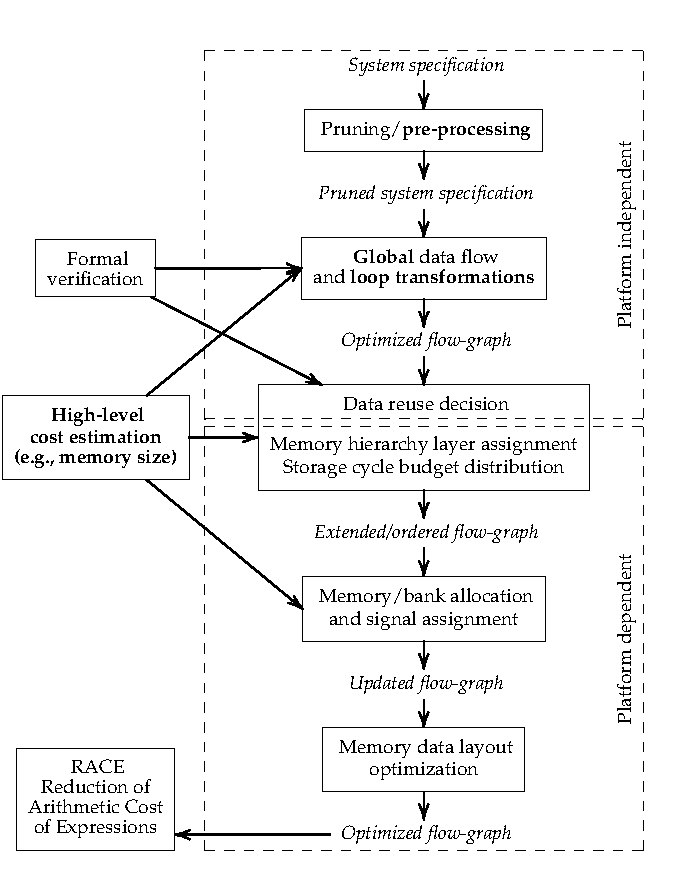
\includegraphics[scale=0.9]{Images/dtse1.pdf}
	\caption{DTSE methodology for data transfer and storage exploration. Source: \cite{palkovicThesis} }
	\label{fig:dtse}
\end{figure}

Platform independent steps of the DTSE reduce the number of array accesses and enable later platform dependent optimization steps. 
They are beneficial for any platform used later in the design-flow and are briefly presented:

\begin{enumerate}

\item Pruning.

This step is necessary to identify and isolate the parts and data structures in the program which are data-dominant and thus relevant for the DTSE. 
The pruning step also presents this code in a way which is optimally suited for transformations. 
Thus mostly loops with large bounds and exhibiting good reuse of data and data structures such as array variables are exposed.
 All the freedom is exposed explicitly, and the complexity of the exploration is reduced by hiding constructs that are not relevant. 
 Apart from areas of power oriented gain, the parts of the program, which are a bottleneck for obtaining better performance need to be identified. 
 These are mostly the data structures that have very little locality but are accessed heavily.
 
 \item Global data-flow transformations.
 
 The goal of the global data-flow optimization step is to reduce the number of bottlenecks in the algorithm that prevent optimizing code restructuring transformations from being applied and remove access redundancy in the data-flow. 
 The transformations consist mainly of advanced signal substitution avoiding unnecessary copies of data, modifying computation order in associative chains enabling certain loop transformations, shifting of delay lines through the algorithm to reduce the storage requirements, and re-computation issues to reduce the number of transfers and storage size. 
 
 \item Global loop and control-flow transformations.
 
 The goal of the global loop and control-flow optimization step is to reduce the global lifetimes of the arrays and to increase the locality and regularity of the data accesses.
  Locality of data accesses means that the accesses to the same memory location have to be close in time and the regularity means that the order of consumption should be the same as the order of production. 
  The transformations remove system-level buffers introduced due to mismatches in production and consumption ordering (regularity problems). 
  They allow also the data to be stored later in the design flow in smaller memories closer to the data paths.
  
  \item Data reuse exploration.
  
The goal of the data reuse decisions step is to better exploit a hierarchical memory organization to benefit from the available temporal locality in the data accesses. 
An important consideration here is the distribution of the data over the hierarchy levels such that frequently accessed data can be read from smaller and less power consuming memories. 
This obviously has a positive effect on the total power consumption of the application because the most frequently accessed data is then read from less power consuming memories. 
Also the smaller memories can then be closer to the data paths thereby reducing the dissipation in the interconnect, especially if off-chip memory accesses are replaced by on-chip memory accesses.
 
\end{enumerate}

Platform dependent steps of the DTSE uses the information about the predefined memory organization to perform further optimizations. 
Some substeps only apply for an (embedded) customizable memory organization which is becoming available on several platforms by partly powering down over-dimensioned memory blocks that are not fully needed. The platform dependent steps are briefly presented:

\begin{enumerate}

\item Memory Hierarchy Layer Assignment (MHLA).

The MHLA step maps the most beneficial candidates from data reuse copy trees to a virtual memory hierarchy subsystem. 
During MHLA, the data reuse copy trees resulting from the data reuse exploration and the corresponding transfers are partitioned over several hierarchical memory layers, based on the bandwidth and high-level memory size estimation. 
The high-level memory class of each of the memory layers is determined (e.g., on-chip, off-chip, ROM, SRAM or DRAM and other RAM “flavors”). 


\item Storage Cycle Budget Distribution (SCBD)

The goal of the SCBD step is to ensure that the (usually stringent) real-time constraints are met with a minimal cost penalty. 
The major substep involves Storage Budget Optimization (SBO) to determine which data should be made simultaneously accessible in the memory architecture such that the real-time constraints can be met with minimal memory bandwidth related costs.
This step mainly determines the bandwidth/latency requirements and the balancing of the available cycle budget over the different memory accesses.
Additional loop transformations are performed to meet the real-time constraints, such as merging of loops without dependencies, software pipelining and partial loop unrolling. 
These loop transformations normally do not influence the access order of data elements, so also the data reuse behavior remains the same.
The data reuse transformations introduce dependencies in the code which constrain the freedom for SCBD transformations. 

\item Memory/bank allocation and signal assignment (MAA).

The goal of the memory allocation and assignment step is to determine an optimal memory architecture for the background data. 
The step allocates memory units and ports (including their types) from a memory library and assigns the data to the best suited memory units, given the cycle budget and other timing constraints. 
The combination of the SCBD and MAA tools allows to derive real Pareto trade-off curves of the background memory related cost (e.g., power) versus the cycle budget.

\item Memory data layout optimization.

In the memory allocation and data-to-memory assignment step, arrays were assigned to physical memories or to banks within predefined memories. 
However, the arrays are still multi-dimensional, while the memory itself knows only addresses. 
In other words, the physical address for every array element still has to be determined. 
This transformation is the data layout decision.
 Main memory data-layout optimization exploits the memory organization data freedom and thus reduces the conflict misses.
For hardware-controlled caches advanced main memory layout organization techniques have been developed, which allow to remove most of the present conflict misses due to the limited cache associativity. % [130].

\end{enumerate}

\section{System Scenarios}

The concept of system scenarios has been presented before in a systematic way on a wide range of applications \cite{GheoThesis}.
This section describes the basic concepts behind the system scenario methodology and its basic steps.
The methodology is applied to a memory specific context in the rest of this thesis. 

The goal of the system scenario methodology is, given an application, to exploit at design time its possible operation modes from the resource usage perspective, without getting into an explosion of details. 
If the environment, the inputs and the hardware architecture status would always be the same, then it would be possible to optimally tune the system to that particular situation. 
However, since a lot of parameters are changing all the time, the system must be designed for the worst case situation. 
Still, it is possible to tune the system at run-time (e.g., change the processor frequency/supply voltage), based on the actual operation mode. 
If this has to happen entirely during run-time, the overhead is most likely too large. 
So, an optimal configuration of the system is selected up front, at design time. 
However, if a different configuration would be stored for every possible operation mode, a huge database is required. 
Therefore, the operation modes similar from the resource usage perspective are clustered together into a single scenario, for which we store a tuned configuration for the worst case of all operation modes included in it.
The system scenario methodology deals with issues that are common: choosing a good scenario set, deciding which scenario to switch to (or not to switch) and using the scenario to change the system knobs. 
This leads to the different steps of the methodology:

\begin{enumerate}

\item Profiling 

This step combines static analysis and profiling of the application and is done at design time.
The studied application is tested exploring the whole range of inputs that is rational for the application.
The system resources and the associated cost are found.
The costs are the resource usage (e.g., number of processor cycles or memory requirements).
 If the information about all possible operation modes in which a system may run is known at design time, and the operation modes are considered in different steps of the embedded system design, a more efficient and effective system may be built, as specific and aggressive design decisions can be made for each operation mode.

\item Identification

In this step, the relevant operation mode
parameters are selected and the operation modes are clustered into scenarios. 
This clustering is based on the cost trade-offs of the operation modes, or an estimate thereof. 
The identification step should take as much as possible into account the overhead costs introduced in the system by the following steps of the methodology. 
As this is not easy to achieve, an alternative solution is to refine (i.e., to further cluster) the scenario identification during these steps. 

\item Detection/Prediction 

At run-time, a scenario has to be selected from the scenario set based on the actual parameter values. 
In general, the parameter values are not known before the operation mode starts, so they have to be estimated, which leads to detection of the scenario. 
Detection is not a trivial task: both the number of parameters and the number of scenarios may be considerable, so a simple lookup in a list of scenarios may not be feasible. 
The detection incurs a certain run-time overhead, which depends on the chosen scenario set. 
Therefore, the scenario set may be refined based on the detection overhead. 

\item Switching

Switching is the act of changing the system from one set of knob positions to another. This implies some overhead (e.g., time and energy), which may be large (e.g., when migrating a task from one processor to another). 
Therefore, even when a certain scenario (different from the current one) is predicted, it is not always a good idea to switch to it, because the overhead may be larger than the gain. The switching step selects at design time an algorithm, which is used at runtime to decide whether to switch or not. 
It also introduces in the application the way how to change the knob positions, and refines the scenario set by taking into account switching overhead.

\end{enumerate}

\subsection{Use-Case vs. System Scenarios}

\begin{figure}[!t]
	\centering
	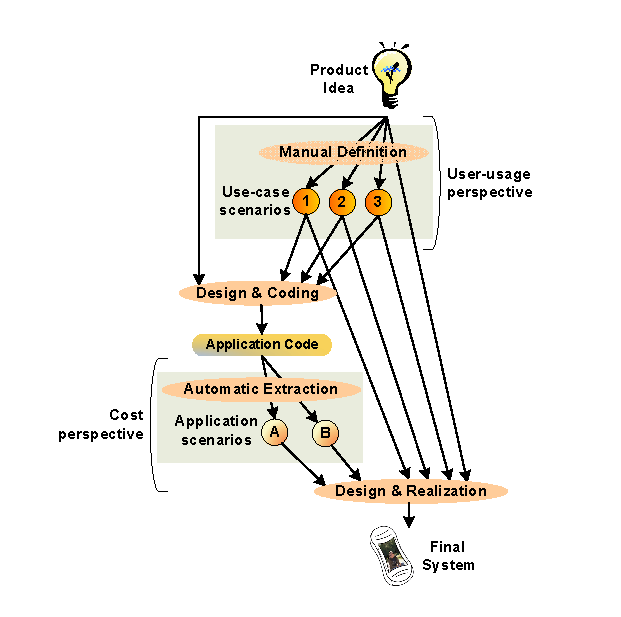
\includegraphics{Images/versus1.pdf}	
	\caption{A scenario based design flow for embedded systems. Source: \cite{GheoThesis} }
	\label{fig:versus}
\end{figure}

Another type of scenario that is used in several published works is the use-case scenario.
Use-case scenario approaches generate different scenarios based on a user's behavior.
These scenarios concretely describe, in an early phase of the development process, the use of a future system. 
In case of human-computer interaction, the scenarios appear like narrative descriptions of envisioned usage episodes, and in case of object oriented software engineering like a unified modeling language (UML) use-case diagram which enumerates, from functional and timing point of view, all possible user actions and the system reactions that are required to meet a proposed system function. 
In the embedded systems area, use-case scenarios are used in both hardware \cite{52} \cite{85} and software design \cite{29}. 
In these cases, the scenarios focus on the application’s functional and timing behaviors and on its interaction with the users and environment, not on the resources required by a system to meet its constraints. 
These scenarios are used as an input during system design for user-centered design approaches.	

This thesis concentrates on system scenarios, which are derived from the behavior of the application. 
These scenarios are used to reduce the system cost by exploiting information about what can happen at run-time to make better design decisions. 
While use-case scenarios classify the application's behavior based on the different ways it can be used, application scenarios classify it from the resource usage perspective, based on the cost trade-off aspects during the mapping to the platform. 
Fig.\ref{fig:versus} depicts a design trajectory using use-case and system scenarios. 
It starts from a product idea, for which the product's functionality is manually defined. 
These scenarios characterize the system from a user perspective and are used as an input to the design of an embedded system that includes both software and hardware components. 
In order to optimize the design of the system, the detection and usage of application scenarios augments this trajectory (the bottom gray box in the figure). 
Once the application is coded, its scenarios related to resource utilization are extracted in an automatic way, and they are considered for the decisions made during the following phases of the system design. 
Hence, the run-time behavior of the application is classified into several application scenarios, where the cost of the operation modes within a scenario is always fairly similar. 
For each individual scenario, more specific and aggressive design decisions can be made.
	
System scenario methodology focuses on the behavior of the system to generate scenarios and can, therefore, fully exploit the detailed platform mapping information. 
In contrast to use case scenario approaches in which scenarios are generated based on a user's behavior, the system scenario methodology focuses on behavior of the system to generate scenarios.
	Furthermore, compared with use case scenario approaches in which scenarios are generated based on a user's behavior \cite{usecase}, the system scenario methodology focuses on the behavior of the system to generate scenarios and can, therefore, fully exploit the detailed platform mapping information.

\section{Scratch-pad Memory Architectures}

Scratch-pad memory architectures are employed in several studies with the objective of improving system performance and energy through means such as reduced memory access count or reduced cache misses. 
Scratch-pad memories provide a good alternative to cache memories due to their higher flexibility.
An example of using partitioning the data variables to scratch-pad memory and DRAM to minimize interference between variables is given in \cite{7}. 
Several examples of clustered memory architectures have been proposed.
In \cite{cho2009adaptive} an adaptive scratch-pad memory is successfully used in order to handle the dynamic behavior of multimedia applications.
In \cite{wang2005energy} a clustered memory architecture is employed and an algorithm is developed, which efficiently uses the memory banks to achieve the maximum energy saving while satisfying the given performance constraint.

%%%%%%%%%%%%%%%%%%%%%%%%%%%%%%%%%%%%%%%
\chapter{Solution Approach}
\label{method}
%make a consistent story about how the papers are connetcted
The proposed solution to the problem expressed in Sec.\ref{sec:problem} is discussed in this chapter.
The solution approach is split into two parts, namely the platform and the methodology.
The first part focuses on the memory architecture in which dynamic applications are executed.
The second part focuses on the necessary steps to efficiently couple the applications and the platform.

\section{Target platform architecture}

Platform architecture is a crucial part of any system scenario methodology.
The platform must provide a set of reconfigurable parameters, known as system knobs, that allow different configurations of the platform.
The different configurations enable the better adaptation of the platform to the requirements of the application for the specific execution.
Many system characteristics can be defined as system knobs and the most common example of such a system knob is the dynamic voltage and frequency scaling (DVFS).
DVFS changes the voltage and the frequency of a processor dynamically.
A lower frequency and voltage is often sufficient to meet the deadline of an application, while the power consumption of the processor is reduced.

\subsection{Target memory platform architecture}

A dynamic memory platform is necessary for the memory-aware system scenario methodology. 
Each configuration of the memory platform corresponds to a different memory energy consumption and available memory space. 
The dynamic memory platform is achieved by organizing the memory area in a varying number of banks that can be switched between different energy states. 
The decision to use memory banks with varying sizes on the clustered memory organization increases the reconfiguration options and consequently the potential energy gains. 
In general, smaller memories are more energy efficient compared to larger memories banks. 
However, in some cases large memory banks are needed in order to fit the application data without the need for too many small memories causing complex interconnects. 
The goal is to use the most energy efficient banks to store the most frequently used data. 

A clustered memory organization with a varying number of memory banks of different sizes is explored.
In  Appendix \ref{norchip} such a clustered scratchpad memory with four banks is introduced. 
It is further expanded to explore memory designs with up to five banks in Appendix \ref{DAES}.

\subsection{Memory models}

The memory models that are used to built the clustered memory architecture heavily influence the design decisions.
The memory architecture consists of the memory banks and the interconnection between the memory banks, which is necessary to connect the memory to the processor.
The most important parameter of the memory models in the current work is the energy profile of the model, although other parameters are also included.
The following models are used in this thesis:
\begin{itemize}
\item Formula-driven memory model presented in \cite{Artes2011}.
The memory energy consumption for every access in the clustered scratchpad memory is calculated using a formula, which takes the size, the number of lines and the word length as input parameters.
The leakage power is calculated in a similar way.
The model supports three different states, namely active, shut-down and retention modes.
This model is presented and employed on the work included in Appendix \ref{norchip}.

\item Commercially available memory macros.  
For those models delay, access energy and leakage power numbers are derived from a commercial memory compiler.
The model supports four different states, namely active, shut-down, light-sleep and deep sleep modes.
This model is presented and employed on the work included in Appendix \ref{DAES}.

\item Experimental standard cell-based memory (SCMEM) \cite{Mei11}.
The standard cell-based memories are synthesized using Cadence RTL compiler for TSMC 40nm standard library. 
Afterwords, power simulations on the synthesized design are carried out using Synopsys PrimeTime, in order to obtain energy numbers.
The model supports four different states, namely active, shut-down, light-sleep and deep sleep modes.
This model is presented and employed on the work included in Appendix \ref{DAES}.

\item Interconnection model based on synthesis results.
The interconnection model is useful in order to estimate the energy consumption in the peripheral logic, outside the memory banks.
This model is developed and presented in the work included in Appendix \ref{interconnection}.

\end{itemize}

There are advantages and disadvantages for each of the used models.
The analytical model is easy to use, has very low computation time and can calculate energy numbers for any possible size of memory, because the input parameters can have any value.
However, the accuracy of the model is lower compared to the other models.
The MM model provides accurate energy numbers, but the designer must rely on a library of memory banks.
The SCMEM model has also high accuracy, as the energy numbers are based on simulation.
The designer has the freedom to develop any desirable configuration, although the process of writing, testing and simulating every new memory design is time-consuming.
Thus, a library of SCMEM is made and the exploration is limited within the already synthesized models.
The interconnection model is normally omitted, because the contribution of the interconnection to the overall energy consumption is very low.
The model is based on synthesis, so it is accurate for the specific synthesized design but the generalization to other designs reduces the accuracy. 

\subsection{Technology scaling}

The proposed clustered memory architecture is an energy efficient platform for dynamic data-intensive applications.
The impact of the technology scaling on the energy efficiency is also explored and presented in Appendix \ref{interconnection}. 
The operationally independent memory banks provide an energy efficient platform, but comes with an interconnection overhead due to the connections between the memory banks. 
The energy consumption on the memory banks is reduced due to the scaling that results in smaller memory cells with lower voltage.
On the other hand, the energy consumption on the wiring follows a slower reduction curve.
Thus, the interconnection energy overhead will increase in the future.
A detailed memory and interconnect energy model is developed that includes the scaling impact.
The model suggests that the proposed target memory platform will continue to be energy efficient.

\section{Data variable based memory-aware system scenario methodology}

The memory-aware system scenario methodology is based on the observation that the memory subsystem requirements at run-time vary significantly due to dynamic variations of memory needs in the application code. 
Most existing design methodologies define the memory requirements as that of the most demanding task and tune the system in order to meet its needs \cite{tcm}. 
Obviously, this approach leads to unused memory area for tasks with lower memory requirements, since those tasks could meet their needs using fewer resources and consequently consuming less energy. 

Designing with system scenarios is workload adaptive and offers different configurations of the platform and the freedom of switching to the most efficient scenario at run-time. 
A system scenario is a configuration of the system that combines similar run-time situations (RTSs). 
An RTS consists of a running instance of a task and its corresponding cost (e.g., energy consumption) and one complete run of the application on the target platform represents a sequence of RTSs \cite{Elena2010}. 
The system is configured to meet the cost requirements of an RTS by choosing the appropriate system scenario, which is the one that satisfies the requirements using minimal power. 

\subsection{Design-time profiling based on data variables}

Application profiling is the analysis of the memory requirements for the studied application and is performed at design-time.
The analysis focuses on the allocated memory size during execution  for a wide range of inputs. 
The profiling stage consists of running the application code with suitable input data often found in a database, in order to produce profiling results.  
The profiling reveals parts of the application code with high memory activity and with varying memory access intensity, which possibly depends on input data variables. 
Because of this behavior, a static study of the application code alone is insufficient since the target applications for this methodology have non-deterministic behavior that is driven by input.

\textbf{!!Luc's question during 2nd oral!!}
The whole set of possible inputs is studied and analyzed, which is timely possible during design-time.
Even a bounded semi-infinite set of input values can be analyzed based on the application's code.
For example, assuming that an input value is any real number in some range, the corresponding memory requirements are calculated by taking the minimum and maximum limits for that range.
The minimum and maximum limits can be found with the help of the application's code.
Thus, the profiling in this case should not be perceived as a training series but rather as a full analysis of the whole input space.
Any possible application input during run-time belong to the input space analyzed during design-time.

Profiling results provided to the designer include complete information about allocated memory size values together with the number of occurrences and duration for each of these memory size values. 
Moreover, correlation between input data variable values and the resulting memory behavior can possibly be observed. 
This information is useful for the clustering step that follows. 
Profiling also reveals the worst case memory usage for a given set of inputs. 
The memory usage is measured using techniques presented in \cite{Ang13b}, in which authors compute the minimum amount of memory resources required to store the elements of an application. 
Appendix \ref{DAES} includes a detailed presentation of this step.

\subsection{Design-time system scenario identification based on data variables}

The scenario identification is the process of organizing the profiled memory sizes into groups with similar characteristics, which are defined as system scenarios. 
Grouping or clustering is necessary, because it will be extremely costly to have a different scenario for every possible size, due to the number of memories needed. 
Clustering neighboring RTSs is a rational choice, because two instances with similar memory needs have similar energy consumption. 
The memory size and the frequency of each RTS are not the only two parameters that should be taken into consideration during the system scenario identification. 
The memory size of each RTS results in a different energy cost depending on the way it is mapped into memory. 
The impact of the different assignment possibilities is included into the clustering by introduction of energy as a cost metric. 
Increasing the number of memory banks results in lower energy per access since the most accessed elements can be assigned to smaller and more energy efficient banks. Unused banks can be switched off.

The system scenario identification step includes the selection of the data variables that determine the active system scenario. 
This can be achieved by careful study of the application code, combined with the application's data input.
The variable selection is done before clustering of RTSs into scenarios.
For the choice of identification variables, there is a trade-off between the complexity and the accuracy of the scenario detection step.
On one hand, if the identification is done using a group of complex variables and their correlation, there is a number of calculations needed in order to predict the active scenario. 
On the other hand, if the value of a single variable is monitored for scenario identification, the scenario detection is straightforward.
Obviously, the accuracy of the scenario detection is higher on the first case, while the computational needs for scenario detection are lower on the second case.
In other words, the more accurate scenario detection, the more resources are used by the run-time manager for detection.

Appendix \ref{DAES} includes a detailed presentation of this step.

\subsection{Run-time system scenario detection and switching based on data variables}

During run-time, all the switching decisions are taken based on the platform and application information. 
In this work, we use a simple and straightforward switching approach.
Memory models provide the necessary information for the switching decision, namely the energy and the time penalty for switching between stages.
The switching step consists of all platform configuration decisions that can be made at run-time, such as the change in the power mode of memory units.
Switching takes place when the switching cost is lower than the energy gains achieved by switching. 
The run-time manager compares the memory energy consumption of executing the next task in the current active system scenario with the energy consumption of execution with the optimal system scenario. 
If the difference is greater than the switching cost, then scenario switching is performed.
Switching costs are defined by the platform and include all memory energy penalties for run-time reconfigurations of the platform, e.g., extra energy needed to change state of a memory unit.

Appendix \ref{DAES} includes a detailed presentation of this step.

\subsection{Interleaving exploration based on data variables}

Interleaving exploration is a complementary technique applied on the application that can further improve energy gains.
Interleaving is a data layout transformation for combining the storage of multiple arrays, so that blocks of data from different arrays are stored contiguously, in order to achieve spatial locality in memory accesses.
By interleaving we are able to group the data to be accessed and thus reduce the number of memory accesses for accessing them.
The basic principles of the performed interleaving exploration are presented in \cite{sharma2013data}.
Interleaving improves the spatial locality and removes redundant data in order to achieve higher  utilization of the hardware resources, especially on single instruction multiple data (SIMD) architectures.

The impact of the data interleaving exploration on the number of memory accesses is significant.
When the accesses are irregular and the data are organized in index order, each memory access results in a small amount of useful data due to the presence of holes.
In contrast the re-organization of the data provides a sequence of useful data without many holes between them.
Thus, a single access to the memory results in a higher number of useful elements.
The overall number of memory accesses is reduced, as each access has a higher utilization.

The goal of the interleaving exploration is to select the optimal set of memory banks and to make  the optimal decision regarding the mapping of the data to the different memory banks.
The parts of the interleaved data that consist mostly of useful elements are mapped into memory banks with low energy per access but at the same time with the necessary access time.
The parts of the interleaved data that consist of access holes and rarely accessed elements are optimally mapped into memory banks with energy efficient retention states.
In both cases the size of  the memory banks should be adequate to fit the stored data but at the same time as small as possible to avoid area and energy penalties.

The interleaving decisions influence the data-to-memory mapping decisions and vice versa.
Assuming that the mapping is performed first using the initial data the following interleaving options are reduced.
For example, the decision to map two arrays on different memory banks removes the option to interleave them later.
Optimizing both the interleaving and the memory mapping at the same time results in a large and inefficient loop of constrain propagation between the two exploration phases.
In other words, the best interleaving solution, which avoid taking into account at all the distributed memory organization, would lead only to a local optimum.
Applying the local optimum to the memory organization results may results in changes due to platform limitations and move to another optimum.
Then, new iterations on data interleaving are maybe needed and so on.
To solve this problem, all the platform parameters are upfront defined and taken into consideration for the interleaving exploration, which is performed first.
Then, the best data interleaving options are propagated to the data-to-memory mapping step.

Appendix \ref{interleaving} presents the full interleaving methodology.

%%%%%%%%%%%%%%%%%%%%%%%%%%%%%%%%%%%%%
\chapter{Research Results and Contributions}
\label{research}

This thesis is a collection of papers that I have authored or coauthored during my time as a PhD student. 
Each paper is presented in the appendix. 
Rather than including the double-column PDF files, I have opted to reformat each paper to increase readability of the graphs and text. 
However, I have not altered the text or figures, only the layout and size.
The order of papers presented here are in rough chronological order and correspond to the different research contributions. 
In practice, some of the research in these papers have been conducted concurrently.

\section{Contribution A: Development of the Memory-Aware System Scenario Methodology}

The main contribution of this thesis is the development of the system scenario methodology for dynamic data-intensive applications.
The methodology provides a systematic way for design-time and run-time handling of the memory subsystem.
The work for the development of the methodology is presented in one journal and two conference papers.

\subsection{Energy Impact of Memory-Aware System Scenario Approach}

\subsubsection{Abstract}

System scenario methodologies propose the use of different scenarios, e.g., different platform configurations, in order to exploit variations in computational and memory needs during the lifetime of an application. In this paper several extensions are proposed for a system scenario based methodology with a focus on improving memory organization. The conventional methodology targets mostly execution time while this work aims at including memory costs into the exploration. The effectiveness of the proposed extensions is demonstrated and tested using two real applications, which are dynamic and suitable for execution on modern embedded systems. Reductions in memory energy consumption of 40 to 70\% is shown.

\subsubsection{Retrospective View}

This work is a case-study of two applications, that strongly motivates the potential gains from using system scenarios in the memory subsystem.
The fact that the chosen applications are from two different domains, supports the effectiveness of the methodology across different domains.
The main ideas of the methodology are presented, although the presentation is heavily coupled with the two case-study examples.

\subsubsection{Roles of the Authors}

I developed the detailed approach and performed the necessary experiments and the writing of the paper, partly based on some initial ideas of Kjeldsberg and Catthoor. 
Hammari provided one of the applications and Huisken helped in the development of the energy model.
I orally presented the paper in the conference.

\subsection{Exploration of energy efficient memory organizations for dynamic multimedia applications using system scenarios}

\subsubsection{Abstract}

We propose a memory-aware system scenario approach that exploits variations in memory needs during the lifetime of an application in order to optimize energy usage. 
Different system scenarios capture the application's different resource requirements that change dynamically at run-time. 
In addition to computational resources, the many possible memory platform configurations and data-to-memory assignments are important system scenario parameters. 
In this work we focus on clustering of different memory requirements into groups and presenting the system scenario generation in detail.
The clustering is a non-trivial problem due to the many different memory requirements, which leads to a very large exploration space.
An extended memory model is used as a practical enabler, in order to evaluate the methodology. 
The memory models include existing state-of-the-art memories, available from industry and academia, and we show how they are employed during the system design exploration phase. 
Both commercial SRAM and standard cell based memory models are explored in this study. 
The effectiveness of the proposed methodology is demonstrated and tested using a large set of multimedia benchmarks published in the Polybench, Mibench and Mediabench suites,
representative for the domain of multimedia applications.
Reduction in energy consumption in the memory subsystem ranges from 35\% to 55\% for the chosen set of benchmarks.

\subsubsection{Retrospective View}

This work is a complete and formal presentation of the methodology work-flow.
The theoretical presentation is accompanied with an extensive number of results for a large set of benchmark applications.
The methodology is both extended and better formulated compared to the previous paper.

\subsubsection{Roles of the Authors}

This work was first presented in embedded systems week, as an oral and poster submission.
Later, it was extended and published as a journal paper.
The main idea is based on the previous paper.
I performed the necessary simulations and wrote the paper, partly based on suggestions and ideas from Kjeldsberg and Catthoor. 

\section{Contribution B: Combined Implementation of the System Scenario Methodology on Memory Subsystem and PEs}

\subsubsection{Abstract}

This work explores the power management options for a transmitting wireless system using system scenarios. We exploit the variations in the communication channel and the protocol requirements during the lifetime of a transmission, in order to optimize energy usage. Both the transmission signal power and the memory subsystem are taken into consideration. Different system scenarios and the corresponding configurations capture the different resource requirements, which change dynamically during transmission. Signal power on the antenna and active memory banks are the two main platform parameters explored in this study and sufficiently detailed system models are presented for both. The trade-off between the accuracy of the generated system scenarios and the switching cost between them is analyzed. The exploration is performed for an increasing number of system scenarios, from 1 to 14, and the reported power gains are over 95\% and over 25\% on the signal power and the memory subsystems respectively.

\subsubsection{Retrospective View}

This work presents the implementation of the system scenario methodology to a wireless system.
The memory-aware methodology developed in this thesis is combined with the general system scenario methodology for processing elements.
The target application is a widely used and recent benchmark.
The exploration includes all the different subsystems and an interesting analysis of the overhead on the scenario generation is presented.
The use of system scenarios in the whole system improves the overall energy efficiency.

\subsubsection{Roles of the Authors}

My contribution on this work is the experimental and the writing part regarding the memory subsystem.
Zompakis did all the experiments and the writing regarding the processing subsystem and the wireless application.
The oral presentation was also performed by Zompakis.
The rest of the authors contributed on the initial idea and the improvement of the text.

\section{Contribution C: Integrated Interleaving and Data-to-Memory Mapping}

\subsubsection{Abstract}

This work presents a methodology for efficient exploration of data interleaving and data-to-memory mapping options for SIMD (Single Instruction Multiple Data) platform architectures.
The system architecture consists of  a reconfigurable clustered scratch-pad memory and a SIMD functional unit, which performs the same operation on multiple input data in parallel. 
The memory accesses contribute substantially to the overall energy consumption of an embedded system executing a data intensive task. 
The scope of this work is the reduction of the overall energy consumption by increasing the utilization of the functional units and decreasing the number of memory accesses.
The presented methodology is tested using a number of benchmark applications with irregularities in their access scheme.
Potential gains are calculated based on the energy models both for the processing and the memory part of the system.
The reduction in energy consumption after efficient interleaving and mapping of data is between 40\% and 80\% for the complete system and the studied benchmarks.

\subsubsection{Retrospective View}

This work is also a combination of the developed methodology and another complementary approach.
The developed methodology is compatible with code transformation techniques and this work focus on the data interleaving.
The integration of the two required some modifications and the final work-flow was tested using a number of benchmarks.
This work suggests that the memory-aware system scenario methodology is complementary to other techniques that improve energy efficiency.

\subsubsection{Roles of the Authors}

The initial idea for this work is partly based on suggestions by Catthoor and the necessary experiments were implemented by me with the help of Sharma.
The majority of the paper was written by me and the rest by Sharma, while all the authors contributed on the further improvement of the text with their feedback.

\section{Contribution D: Interconnection Cost Modeling and Scaling}

\subsubsection{Abstract}
Power consumption is the key limitation in modern embedded devices.
The memory architecture contributes significantly on the overall power consumption of the system.
Among other proposed techniques, one effective system design approach to reduce the memory power needs is the design of a dynamically reconfigurable clustered memory architecture.
The operationally independent memory banks provide an energy efficient platform, but comes with an interconnection overhead due to the connections between the memory banks. 
Thus, there is a trade-off between the energy gains by increasing the number of memory banks and the increase on the interconnection overhead.
This work explores the future development of the interconnection overhead, as the interconnection cost is expected to increase while the process technology shrinks to 5nm.
The current study employs both CAD tools with simulation results using the current technology and projections provided by institutions.
We use predictive technology models and the quantitative data are supported partly by information
from ITRS and IMEC's interconnect technologists.
A model is developed that provide a sufficiently accurate estimation about the interconnection cost overhead for clustered memory architectures consisting of two to five memory banks and a range of technologies from 40nm to 5nm.  

\subsubsection{Retrospective View}

This work investigates the effectiveness of the memory-aware system scenario methodology in the future.
A reconfigurable memory architecture is a requirement for the implementation of the methodology, thus it is important to study the development of similar architectures in the future. 

\subsubsection{Roles of the Authors}

I performed the necessary development work and wrote the paper, partly based on suggestions from Kjeldsberg and Catthoor. 

%%%%%%%%%%%%%%%%%%%%%%%%%%%%%%%%%%%%%
\chapter{Conclusions and Future Work}
\label{conclusions}

\section{Conclusions}

The main scope of this dissertation is to develop a system scenario methodology that focuses on memory organization. 
The developed methodology exploits memory requirement variations and achieves significant reduction of memory energy consumption, which is of great importance in embedded devices. Since memory size requirements are still met in all situations, performance is not reduced. 
The memory-aware system scenario methodology is suited for applications that experience dynamic behavior with respect to memory organization utilization during their execution.
A wide range of application domains, including multimedia, wireless and bio-medical applications, are tested to prove the effectiveness of the methodology.

An extensive memory energy model is developed in order to have sufficiently accurate simulations and results.
A library is built based on commercial and experimental state-of-the-art memory models.
The library is employed for the construction of reconfigurable memory architectures, which are suitable for the implementation of system scenarios.
Another model is developed to study the impact of the interconnect on the overall energy.
The model suggests that overhead will be kept low in the short term and will increase within reasonable levels in the mid-long term.
Therefore, the design of energy efficient clustered memory architecture will continue to be a good design choice.

Apart from justifying the effectiveness of the system scenarios methodology on the memory, this work explores the compatibility of the methodology with other techniques.
Firstly, the application of the system scenarios methodology in the complete system, including the memory and the processing subsystem, is studied.
Secondly, the proposed methodology is integrated with code and data transformation techniques.
A methodology for efficient exploration of data interleaving and data-to-memory mapping options is developed and tested.
A wide range of applications is studied that allow us to draw conclusions about different kinds of dynamic behavior and their effect on the energy gains achieved using the methodology. 

\section{Future Work}

The future research to improve the current work can focus on the system scenario methodology and/or the memory models and architectures.

One improvement is to fully automate the memory-aware system scenario methodology.
The optimal implementation should take as an input the application code and the library of memory models and automatically generate the most energy efficient memory architecture.
In the current work several scripts were developed to speedup the design space exploration, but the work-flow is not fully automated.
The improvement of the prediction and the identification phase of the methodology could be another significant contribution. 
A multidimensional scenario clustering for the whole system is an interesting improvement.
The N-dimensional exploration space will include several parameters, such as memory energy, PE energy, execution time and reliability, and new methods should be developed to handle the explosion of the exploration space.

The accuracy of the energy models can be significantly increased.
More detailed models can be developed based on an extensive research and simulation.
All the possible clustered memory architectures can be synthesized and tested to get a detailed report on the energy numbers, although it is a very time consuming task.
Especially the interconnect model can be extended by taking the delay into consideration and the synthesis of more designs can steer the model.
A manually improved placing and routing strategy will provide more accurate results regarding the overhead for clustered memory architectures.
An architecture with point-to-point connections between all or some of the memory banks could be explored. 
Such an architecture allows the direct transfer of data between the memory banks without the intervention of the processor.
The data transfers between the memory banks may be useful in some cases, although the interconnection overhead is expected to increase significantly.

\addcontentsline{toc}{chapter}{Bibliography}	
\bibliographystyle{plain}
\bibliography{reference}
